\documentclass{my_cv}
\usepackage[left=3cm,right=3cm,top=1cm,bottom=1cm]{geometry}
\usepackage{fontawesome}
\usepackage{graphicx}
\usepackage{url}
\begin{document}
	\noindent
	\begin{minipage}[t]{.5\linewidth}
		\raggedright 
		\vspace{-2cm}
		{\bfseries \Huge Zhihao Yao}\\
		\small\itshape
		\faHome \hspace{1mm}  Elsterstraße 12, 04109, Leipzig\\
		\faMobilePhone\hspace{1mm} +49-151-12734936\\
		\faEnvelopeO \hspace{1mm} zyao2015inf@gmail.com\\
	\end{minipage}
	\begin{minipage}[t]{.5\linewidth}
		\raggedleft 
		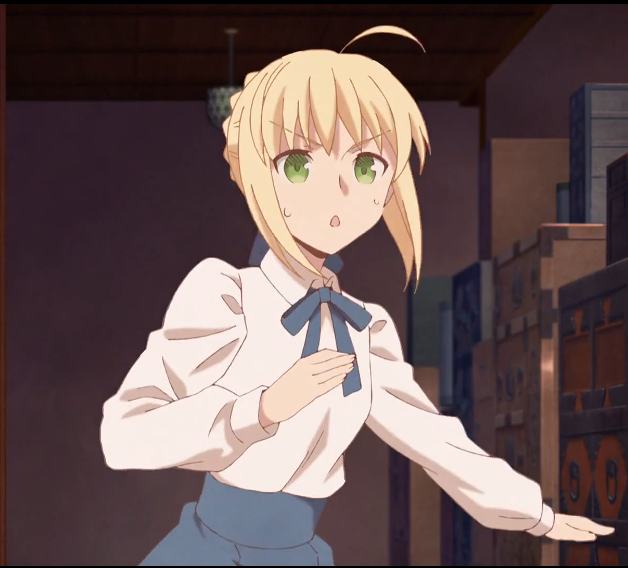
\includegraphics[width=.4\linewidth]{saber_moe.png}
	\end{minipage}
	\section{\faMale\ Personal Description}
	My fullname is Zhihao Yao, I was born on 29.07.1993 in Maanshan, a city situated in the south-east of China. After a successful master study major in Computational Logic, TU Dresden, I believe I have qualifications for both practical and theoretical tasks related to Semantic Web.
	\section{\faGraduationCap\ Education}
	\datedsubsection{Technische Universität Dresden}{2015--2019}
	Master of Science, Computational Logic, graduate with the final grade of 1.7.
	\datedsubsection{Anhui University of Technology}{2011--2015}
	Bachlor of Engineering, Computer Science and Technology, graduate with the final grade of 2.0 (According to the German grading system). 
	\section{\faBriefcase\ Experience}
	\datedsubsection{Exchange Student}{2016.2--2016.7}
	A half-year study at the {\itshape Free University of Bolzano, Italy}. 
	\datedsubsection{Teaching Assistant}{2017.1--2017.2}
	Tutor of the course {\itshape``Science of Computational Logic"}, organise the exercise as well as help checking exam papers. It is a student contract with the Research Group {\itshape``Knowledge Representation"} in TU Dresden.
	\section{\faFolderOpen\ Project}
	\datedsubsection{OWL2TPTP}{2017.4--2017.11}
	A JAVA program to translate OWL files into files in TPTP (Thousands Problems of Theorem Proving) format, then with the help of first-order model finders, we can compute the minimal model under a given fixed-domain. This project was carried out under the supervisation of the Research Group "Computation Logic" in TU Dresden.\\
	\faGithub\  \url{https://github.com/ZhYao2015/2017summer/tree/master/owl2tptp}
	\datedsubsection{An ASP-Based SPARQL Query Engine}{2018.4--2018.12}
	A corresponding JAVA implementation of my master thesis. Broadly speaking, we solve the task of answering SPARQL Query over Datasets by translating both Datasets and Queries into Answer set programs. For ontologies, we can compute the certain answer under a so-called fixed-domain semantics. The translation of Ontologies is an independent work of ``Computational Logic" Group in TU Dresden.\\
	\faGithub\ \url{https://github.com/ZhYao2015/sparql-experimental}
	\section{\faKey\ Skills}
	\begin{itemize}
		\item Artificial Intelligence: Description Logics, OWL, SPARQL, Machine Learning
		\item Others: Java, HTML/CSS/JS, \LaTeX
	\end{itemize}
	\section{\faGlobe\ Languages}
	\vspace{-5mm}
	\begin{table}[h]
		\begin{tabular}{lll}
			{\bfseries \Large Chinese}&{\bfseries \Large English}&{\bfseries \Large German}\\
			Native speaker & Proficient & Basic\\
		\end{tabular}
	\end{table}
\end{document}